% !TEX root = ../main.tex
\chapter{Experiments and results}
In this chapter will be outlined the experimentation phase of the project.
The experimentation has been divided in two types. The first one assessed the performance of the model platform and the reasoner whilst the second one has been the development of a functioning proof of concept of a conversational natural language interface.
Each section will describe the setup and the result of one of the experimantations trying to interpret the results.
\section{Reasoner performance}
For the sake of performance evaluation KITT has been deployed on a local liberty webserver, simulating the cloud based running environment of real deployments.
The performances have been evaluated in respect to the two classical measures, time and space requirements. Since real case scenarios for commercial buildings have considerably larger dimensions than the examples presented in previous chapter and that deployment data of real case wasn't available due to privacy reasons, in order to run a simulation that likely reflect real world data, the following route has been taken.
A given architecture, representing a floor of a building, has been repeated over and over until reaching the complexity of a two hundred storeys building, each of which is comprised of up to a hundred rooms. For comparison, the tallest building in the world, as of 2018, is the Burj Khalifa in Dubai with 163 storeys. From \autoref{fig:experiment_single} it can be seen the structure of the first synthetic example of the test building. Every room is equipped with four Points: a temperature sensor, an occupancy sensor, a cooling valve command and a heating valve command. The rooms are located to the side of a corridor and are adjacent up to by two. This configurations represent a floor. Floors are then stacked one upon the other to form the final building. The outside environment is supposed to monitored by a temperature sensor and an illumination sensor.
\begin{figure}
  \centering
  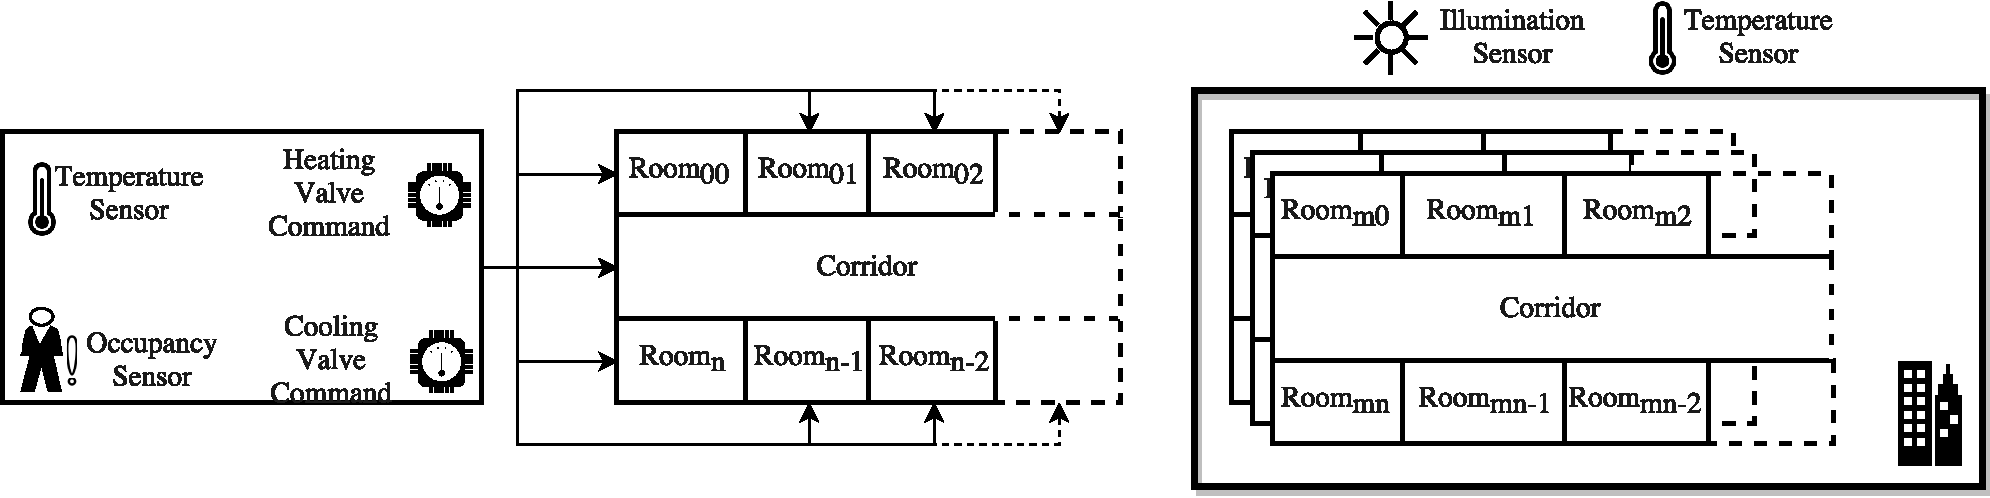
\includegraphics[width=\textwidth]{experiment_simple.pdf}
  \caption{Construction of experiment data}
  \label{fig:experiment_single}
\end{figure}
Given this configurations a full stack of reasoning rules are executed so that a physical model can be derived. The rules can be seen in %TODO append rule.

\begin{table}
\centering
\caption{Performance test result for the simple model}
\label{tab:perf_simple}
\begin{adjustbox}{max width=\textwidth}
\begin{tabular}{lll|llll|llll}
\textbf{Floors} & \textbf{Rooms} & \specialcell{\textbf{No.}\\\textbf{Sensors}} & \textbf{Vertexes} & \textbf{Edges} & \specialcell{\textbf{Vertexes}\\\textbf{reasoning}} & \specialcell{\textbf{Edges}\\\textbf{reasoning}} & \specialcell{\textbf{Memory}\\\textbf{create}\\\textbf{{[}MB{]}}} & \specialcell{\textbf{Memory}\\\textbf{reasoning}\\\textbf{{[}MB{]}}} & \specialcell{\textbf{Time}\\\textbf{create}\\\textbf{{[}ms{]}}} & \specialcell{\textbf{Time}\\\textbf{reasoning}\\\textbf{{[}ms{]}}} \\\hline
1 & 1 & 10 & 123 & 381 & 143 & 477 & 8 & 54 & 16 & 95 \\
1 & 10 & 46 & 168 & 588 & 251 & 1008 & 10 & 98 & 18 & 166 \\
1 & 100 & 406 & 618 & 2658 & 1331 & 6318 & 47 & 228 & 156 & 2047 \\
10 & 10 & 82 & 672 & 2973 & 1448 & 7011 & 53 & 151 & 186 & 2587 \\
10 & 100 & 442 & 5172 & 24483 & 12248 & 61731 & 169 & 300 & 15850 & 256934 \\
20 & 100 & 482 & 10232 & 48733 & 24496 & 48733 & 62 & 284 & 73692 & 1352861 \\
50 & 100 & 602 & 25412 & 121483 & 60768 & 308011 & 143 & 267 & 492255 & 12631754 \\
80 & 100 & 722 & 40592 & 194233 & 97158 & 492721 & 261 & 416 & 1312923 & 34668894 \\
100 & 100 & 802 & 50712 & 242733 & 121418 & 615861 & 194 & 510 & 2172877 & 54904640 \\
200 & 100 & 1202 & 101312 & 485233 & 242718 & 1231561 & 922 & 1014 & 8742782 & 225609628
\end{tabular}
\end{adjustbox}
\end{table}
\begin{figure}
  \centering
  \begin{tikzpicture}
  \begin{axis}[
    legend style={font=\small},
    legend pos=north west,
    xlabel=No. Sensors,
    ylabel=No. Vertexes]
  \addlegendentry{(No.Sensor, Vertexes)}
  \addplot table [y=V, x=Ns]{res/simple_table.txt};
  \addlegendentry{(No.Sensor, Edges)}
  \addplot table [y=E, x=Ns]{res/simple_table.txt};
  \end{axis}
  \end{tikzpicture}
  \caption{Correlation between the number of sensors and the graph vertices and edges count}
  \label{fig:sensor_vertexes_chart}
\end{figure}
\begin{figure}
  \centering
  \begin{tikzpicture}
  \begin{axis}[
    legend style={font=\small},
    legend pos=north west,
    xlabel=Vertexes,
    ylabel=Memory]
  \addlegendentry{(Vertexes, $Mem_{c}$)}
  \addplot table [y=MEMC, x=V]{res/simple_table.txt};
  \addlegendentry{(Vertexes, $Mem_{r}$)}
  \addplot table [y=MEMR, x=V]{res/simple_table.txt};
  \end{axis}
  \end{tikzpicture}
  \caption{Correlation between the number ground truth vertices and the reasoning memory usage}
  \label{fig:vertexes_mem_chart}
\end{figure}
both the experiments shown that even though the graph dimension augments linearly with the number of sensor in a building, as well as the memory needs, that increase with the dimension of the graph,
